\documentclass{article}
\usepackage[utf8]{inputenc}
\usepackage{graphicx}
\usepackage{multicol}
\newcommand\tab[1][.5cm]{\hspace*{#1}}
\setlength{\parindent}{0pt}

\title{Final}
\author{CSE4510: Software Reverse Engineering Section 01\\
	Professor: Christopher Stricklan \\
	Eric Pereira}
\date{May 3, 2019}

\begin{document}
	
	\maketitle
	
	\tab To start, we are given two files for the final and these hold a flag we are supposed to catch. There are two stages to this final so we will start with stage 1:
	
	\subsection*{Stage 1}
	\tab Stage 1 starts by asking for a login id. The login id is pretty simple, it is our standard 
	Florida Tech usernames, so my username is: \textbf{epereira2015}. After that it has an empty line and
	if you give it another newline character it will go to what is the failcase; \texttt{Snoogins}.
	\begin{center}
		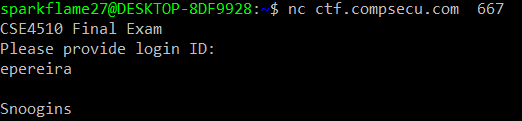
\includegraphics[scale=0.5]{Stage1BlankFail.png}
	\end{center}
	\tab I went to explore the binary to see what the issue was. I explored the binary of the
	\texttt{finalexam} executable. I started down the rabbit hole, which started with the \texttt{main}.
	following the \texttt{main} led me to the \texttt{exam} function, and the first call in this after the
	login id is the \texttt{Stage1Check} function. This function had a peculiar function, the \texttt{hash}
	function, which is displayed below, showing the logic.
	\begin{center}
		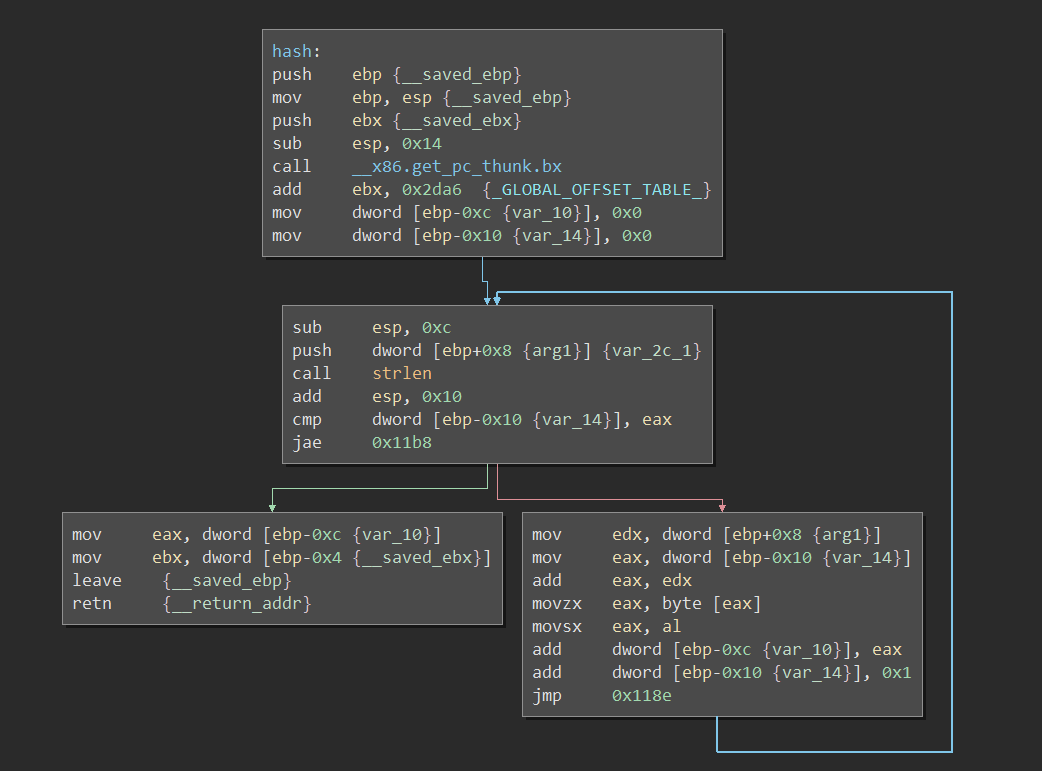
\includegraphics[scale=.45]{hash.png}
	\end{center}
	\tab Essentially what this does is it loops as many times as there are letters in \texttt{arg1}, and
	\texttt{arg1} is the login id you input. What it does in the loop is it gets the ASCII value of each
	letter in the submitted login id and it adds them together. For my username this means that I need to 
	get the character value of each letter/symbol in the name and add them together. If I add each letter in
	my login id together I get the value 1045 and upon testing it out I get a result that brings me to a checkerboard! \\
	\tab It is also important to note there is an error if you do not user the right login id. If the login 
	id that is used does not exist as a \texttt{.so} file in the libraries it will not pass stage 1, as the
	example below shows:
	\begin{center}
		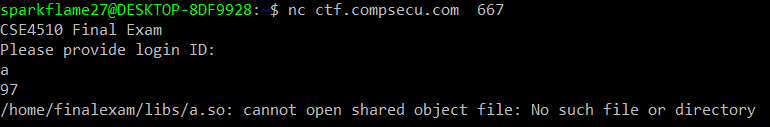
\includegraphics[scale=0.6]{Stage1BadSo.png}
	\end{center}
	
	\subsection*{Stage 2}
	\tab Stage 2 starts with a game of Connect 4. This game of Connect 4 asks for Player X's input, Player X
	being me, the user, and once I give a number coordinating to a specific column a response will come
	from Player Y, an automated bot. This game is actually relatively easy, I discovered that 
	the bot plays the same exact moves each time. This makes it relatively easy to win. Winning provides a 
	screen that looks like:
	\begin{center}
		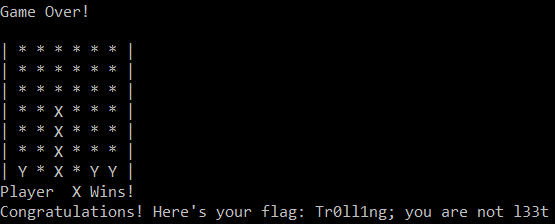
\includegraphics[scale=.6]{TrollFlag.png}
	\end{center}
	\tab This is very clearly a Ben Kenobi ``These aren't the flags you are looking for" moment. This meant
	it was time to go down the rabbit hole of the binary. I went into the \texttt{Stage2} function, and 
	immediately saw the check I mentioned in the previous \textbf{Stage 1} section, where I realized I could
	not simply use any username but only login id's with matching \texttt{.so} files in the libraries. I then
	decided that the issue be in my \texttt{.so} file, as \texttt{Stage2} seems to end right there, and not
	do too much, so I went to my \texttt{epereira2015.so} to see if anything there could give me a hint as
	to what exactly is going on. I started by going into the \texttt{StartGame} function. Reviewing this
	function I noticed there were calls to an object called \texttt{Logger}, which I assumed was a way to 
	log my moves so that maybe the bot could make its decision, but I thought that didn't make sense either
	because it seemed to play the same moves no matter what I did. I found it strange, but let it continue. 
	Upon the continuation of this I noticed a \texttt{success} and scrolling down I saw a string that would
	print a string with what would be my flag. Strange, I did not see it write when I ran it though, maybe it
	is a special case? That did not seem to make too much sense. Then I noticed something strange, very strange, and this led me down another rabbit hole. This is when I saw the result was printing to the
	\texttt{Logger}!
	
	\begin{center}
		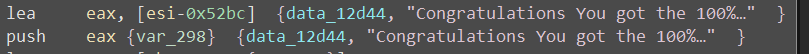
\includegraphics[scale=.8]{StringIWant.png} \\
		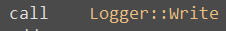
\includegraphics[scale=1]{LoggerWrite.png}
	\end{center}

	\tab Upon this discovery I was confused as to where exactly the \texttt{Logger} was writing to, I needed
	access to it somehow. I went back to see if there were any hints as to exactly what I needed. In the 
	\texttt{StartGame} function I was looking through to see if there were any calls to the \texttt{Logger}
	, and there was one distinct call I noticed, one that seemed it would be important as it opened a new
	Socket. I went to see in the \texttt{OpenSocket} call in \texttt{Logger}, and went exploring through
	each function inside it. I noticed that there was a number being pushed with an string, a string saying
	open socket.
	\begin{center}
		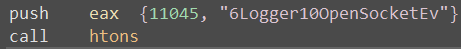
\includegraphics[scale=1]{11045BINGO.png}
	\end{center}
	\tab This number, 11045, is the number I believed to be the socket number, and it looked suspicious as 
	well because it was my hash number (1045) added to 10,000. Upon testing however, I ran into a few
	problems, I believed they may have been server side, I am uncertain as to how many people in the class
	have also experienced this problem. I got strange output in the log that looked like:
	\begin{center}
		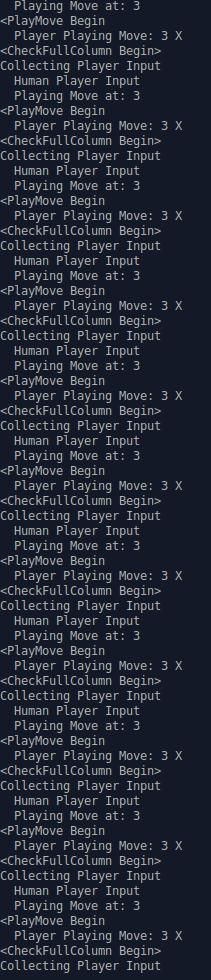
\includegraphics[width=4cm, height=17.5cm]{what.jpg}
	\end{center}

	\tab This is before I put in anything, not to mention I usually press ``2" because my specific bot allows
	me to win if I type ``2" four times in a row. I eventually got 1 working piece with my flag, however I
	had to use a friends VPS (I believe something is wrong with the connection in some way because it worked
	through the VPS but not my laptop), the result I found was this:
	\begin{center}
		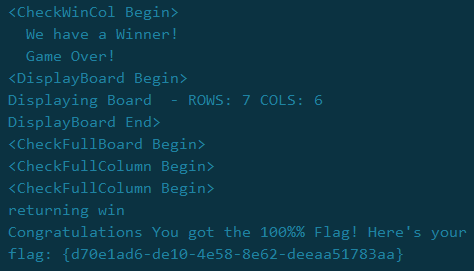
\includegraphics{WinnerFlag.png}
	\end{center}

	\tab Although going through a friends VPS worked, I was unable to create and write a script including 
	this (I was not able to use his VPS for long, and did not work with the script much there). My script
	allowed me to pass Stage 1 and get the Stage 2 \texttt{Tr0lling} flag, but I am unable to really read
	the log files and as a result my script does not output anything for the second flag. I wrote some 
	information in the notes as to ideally what I would use to print out my results in the log, but as 
	mentioned previously, it seems that I was unable to completely test or write a decent script for this. 
	
\end{document}